 
  \section{Examples}\label{sec:examples}
	This section showcases typical use cases for the \tiger IDE. 
	
	\subsection{Creating a new \tiger Language Definition}
	
	The usage of the \emph{New Tigerseye Language Definition} wizard will be explained by creating a \emph{Trivalent-DSL}. A
	Trivalent logic DSL adds an \texttt{unknown (U)} value to the boolean values \texttt{true (T)} and \texttt{false (F)}, so \texttt{T\&U} is U and \texttt{T|U} is T and so on.
	
	\begin{itemize}
	 \item First create a new Java Project. This Project will contain the Trivalent language created by the wizard. In this example a project called \texttt{de.tud.stg.tigerseye.examples.trivalent} will be created
	 \item Right Click on the Project and choose \emph{New > Other}.
	 \item Choose \emph{Tigerseye Language Definition} in the \emph{Tigerseye} folder (Figure \ref{fig:new_tiger_lang}).
	 \item Each language definition consists of a Groovy class that defines all operations, literals and structured elements of the DSL. Type \texttt{TrivalentDSL} as the class name, \texttt{de.tud.stg.tigerseye.examples.trivalent} as the package and select \emph{Next} (Figure \ref{fig:example_newlang_newlangclass}).
	 \item Now add three new literals: \texttt{T} (true), \texttt{F} (false) and \texttt{U} (unknown). They are all of type Trivalent (Figure \ref{fig:example_newlang_literalsadded}). After finishing the wizard these three classes and the supertype Trivalent will be created. Notice that T, F and U extend Trivalent.
	\item The only operation will be an enhanced println which takes a String and a Trivalent expression and prints both, e.g. \texttt{puts("T|U: ",T|U)} will produce \texttt{T|U: T}. The return type should be \texttt{void} so we just let the \texttt{Return type:} field empty. For each operation you can choose if setting a breakpoint on a line containing this keyword should be possible (Figure \ref{fig:example_newlang_operationadded}). Also you can define all parameters and their types.
	\item Now add a repeat-statement. The following will simply print \texttt{T: T} ten times to stdout.
	  \begin{verbatim}	  
repeat(10) {
  puts("T:",T);
}
	  \end{verbatim}
	The return type will be \texttt{void} and there is one parameter named \texttt{n}. Select \texttt{explicit parameters} (Figure \ref{fig:example_newlang_structuredelementadded}).
	Again, you can choose if it should be possible to set a breakpoint on a line containing this keyword.
	\item After you select \texttt{Finish} a dialog will pop up asking you if you want to add the \tiger runtime libraries (Figure \ref{fig:example_newlang_addruntime}). Usually you should say yes, since language definitions have dependencies to the runtime libraries.
	\item The final result is shown in Figure \ref{fig:example_newlang_generatedcode}. For the new type \texttt{Trivalent} as well as for the literals \texttt{T,U and F} a separate Groovy class is created. The language configuration is defined in the \texttt{TrivalentDSL} class.
	\end{itemize}

	\begin{figure}
	  \centering
	  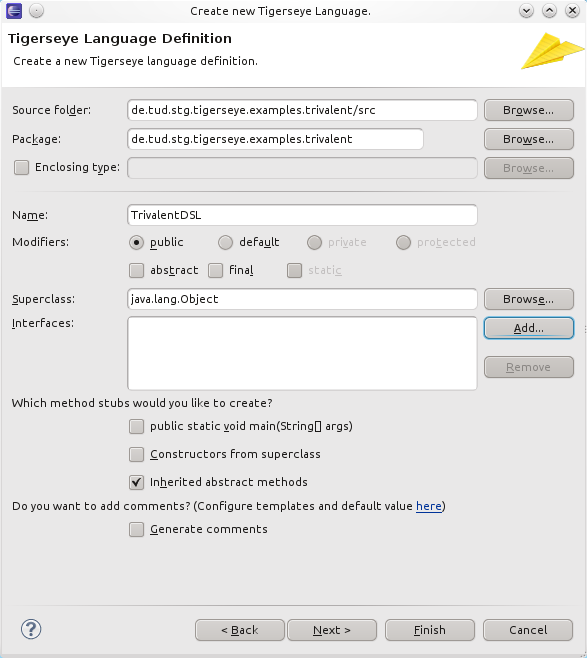
\includegraphics[width=.5\textwidth,keepaspectratio=true]{./pics/example_newlang_newlangclass.png}
	  \caption{New TrivalentDSL Language Defintion}\label{fig:example_newlang_newlangclass}
	\end{figure}

	\begin{figure}
	  \centering
	  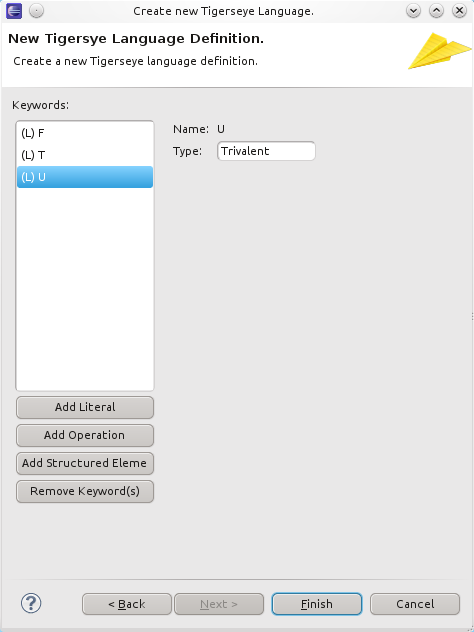
\includegraphics[width=.5\textwidth,keepaspectratio=true]{./pics/example_newlang_literalsadded.png}
	  \caption{TrivalentDSL Language Definition with Literals added}\label{fig:example_newlang_literalsadded}
	\end{figure}
	
	\begin{figure}
	  \centering
	  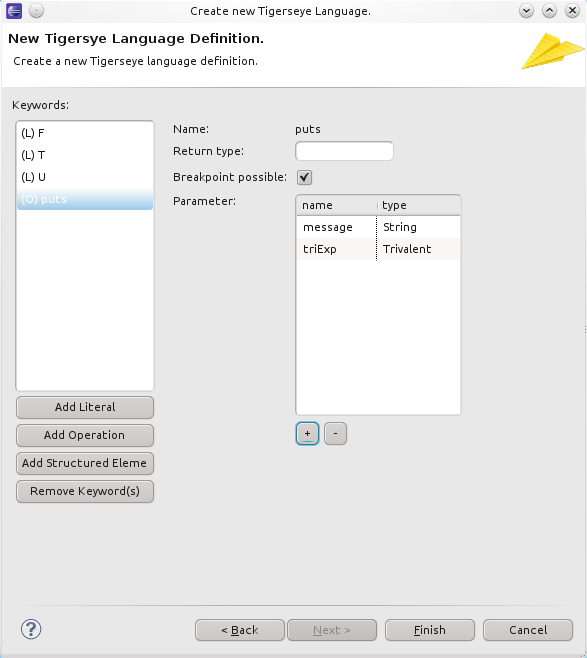
\includegraphics[width=.5\textwidth,keepaspectratio=true]{./pics/example_newlang_operationadded.png}
	  \caption{TrivalentDSL Language Definition Operation \texttt{puts} added}\label{fig:example_newlang_operationadded}
	\end{figure}
	
	\begin{figure}
	  \centering
	  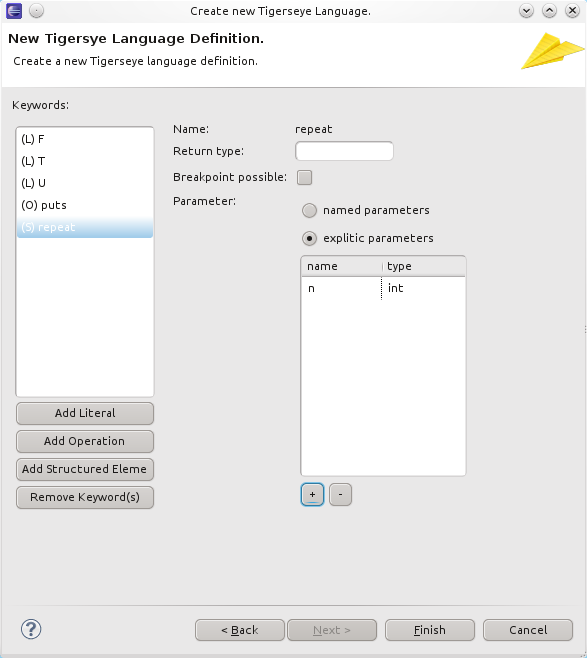
\includegraphics[width=.5\textwidth,keepaspectratio=true]{./pics/example_newlang_structuredelementadded.png}
	  \caption{TrivalentDSL Language Definition Structured Element \texttt{repeat} added}\label{fig:example_newlang_structuredelementadded}
	\end{figure}
	
	\begin{figure}
	  \centering
	  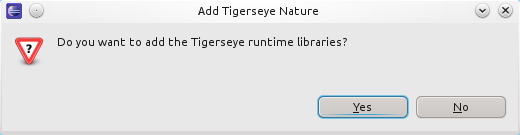
\includegraphics[width=.5\textwidth,keepaspectratio=true]{./pics/example_newlang_addruntime.png}
	  \caption{Question Dialog to add \tiger Runtime Libraries}\label{fig:example_newlang_addruntime}
	\end{figure}

	\begin{figure}
	  \centering
	  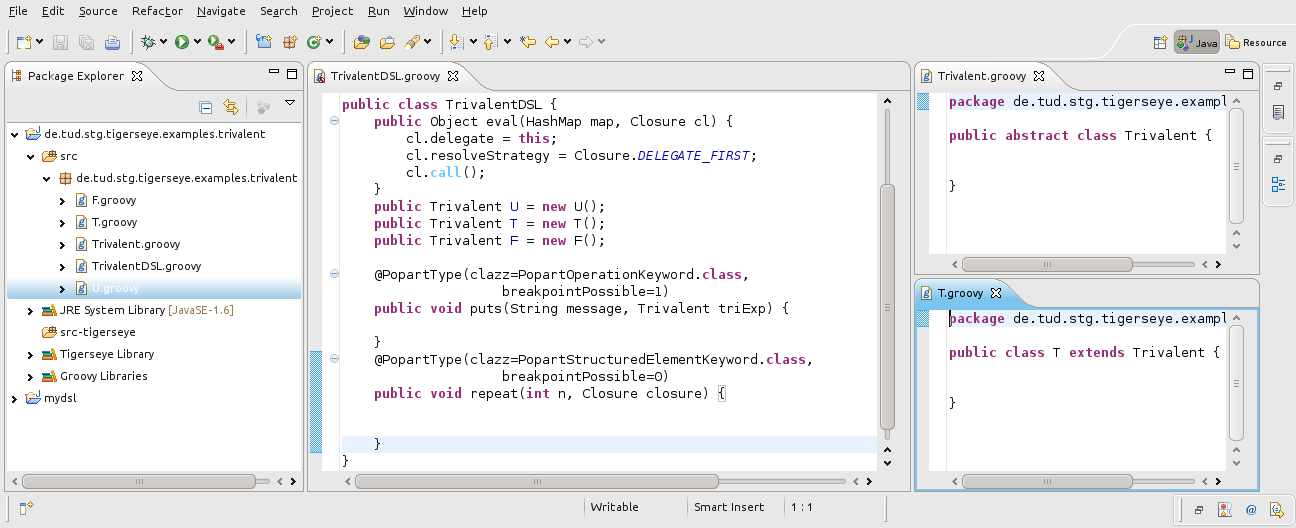
\includegraphics[width=\textwidth,keepaspectratio=true]{./pics/example_newlang_generatedcode.png}
	  \caption{TrivalentDSL Generated Classes and Code}\label{fig:example_newlang_generatedcode}
	\end{figure}

  \subsection{Deployment of a \tiger Language}
  
  To deploy a new language s.t., the user converts his designed language to a plug-in project. This plug-in project will declare its dependencies to two \tiger plug-ins:
  \begin{itemize}
   \item \texttt{de.tud.stg.tigerseye}
   \item \texttt{de.tud.stg.tigerseye.eclipse.core}
  \end{itemize}
  The \texttt{de.tud.stg.tigerseye} plug-in provides the dependent on libraries and the \texttt{de.tud.stg.tigerseye.eclipse.core} plug-in the extension which declares that this plug-in project actually provides a new language.
  
  The following steps have to be performed:
  \begin{enumerate}
   \item Convert the language definition project to a plug-in project. (Figure \ref{fig:example_deploy_converttoplugin})
   \item In the \texttt{MANIFEST.MF} file add the dependencies to the two Tigerseye plug-ins. (Figure \ref{fig:example_deploy_addplugindependencies})
   \item Now open the \texttt{plugin.xml} and go the \texttt{Extensions} tab. Add the \texttt{de.tud.stg.tigerseye.dslDefinitions} extension point. On the extension point select \texttt{New > language}. There you can define the language class to be used. In this example this would be \texttt{de.tud.stg.tigerseye.examples.trivalent.Trivalent}. Additionally you should define a user friendly name of your new language, e.g. \emph{Trivalent DSL}. Optionally you can define the default extension identifying your language, such as \texttt{tri}. Figure \ref{fig:example_deploy_extensionpoint} shows the example configuration. The extension can also be configured using the \tiger preference pages.
   \item Currently only the deployment for development is supported. Language can either be copied or linked inside the eclipse instance in which the \tiger plug-in is developed. The next time the \tiger Eclipse instance is started the language will be visible in the preference pages and can be used.
%    \item Now you can use the export functionality to export the language as a plug-in into a separate jar-file. This can then be copied either into Eclipse's \texttt{dropins} folder or into the \texttt{plugins} folder.
%    \item After a final restart the language should be visible in the languages preference page.
  \end{enumerate}

  	\begin{figure}
	  \centering
	  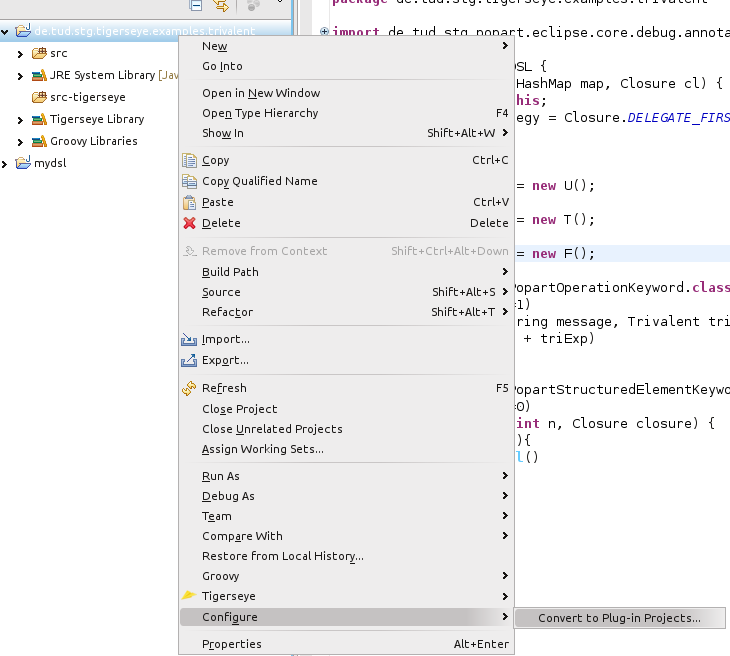
\includegraphics[width=.5\textwidth,keepaspectratio=true]{./pics/example_deploy_converttoplugin.png}
	  \caption{Add Plug-in Project Nature}\label{fig:example_deploy_converttoplugin}
	\end{figure}
	 
	\begin{figure}
	  \centering
	  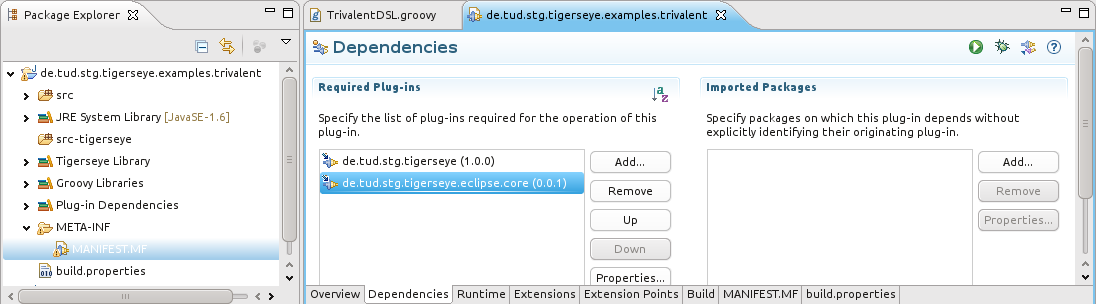
\includegraphics[width=\textwidth,keepaspectratio=true]{./pics/example_deploy_addplugindependencies.png}
	  \caption{Add Plug-in Depedencies to \tiger}\label{fig:example_deploy_addplugindependencies}
	\end{figure}
	
		\begin{figure}
	  \centering
	  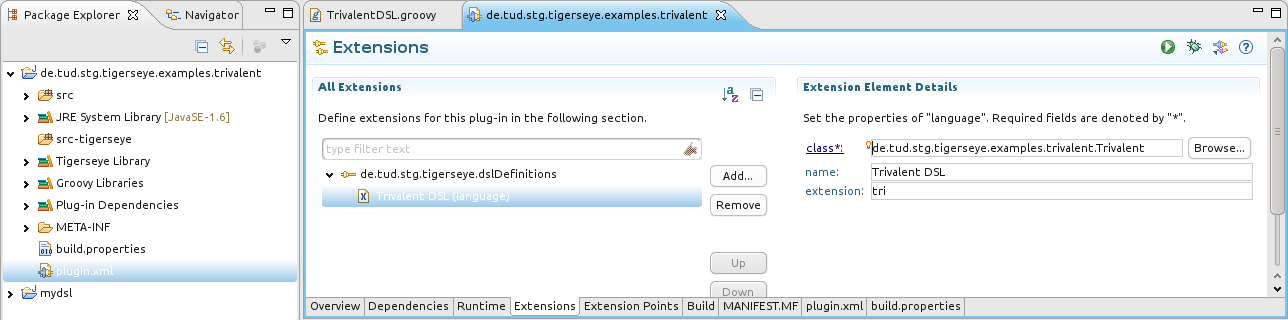
\includegraphics[width=\textwidth,keepaspectratio=true]{./pics/example_deploy_extensionpoint.png}
	  \caption{\texttt{dslDefinitions} Extension Point Configuration}\label{fig:example_deploy_extensionpoint}
	\end{figure} 
